\documentclass[11pt]{article}

\usepackage{amssymb,amsmath}
\usepackage{times,psfrag,epsf,epsfig,graphics,graphicx,caption}
\usepackage{enumitem,fontawesome}
\usepackage{algorithm}
\usepackage{algorithmic}

\begin{document}
\date{}

\title{PHSX 343: Assignment 11}

\author{William Jardee}

\maketitle


\section*{Problem 1}
    This homework seemed to be mostly plug-and-chug, so enjoy the list of equations:
    \[e = \sigma T^4 = \frac{P}{A_s} = \frac{P}{4 \pi r^2}\]
    \[\lambda _{max} T = 2.898 \times 10^{-3} = \gamma \rightarrow \frac{\gamma}{\lambda} = T\]
    \[\frac{P_{tot}}{4 \pi r^2} = \sigma T^4\]
    \[r^2 = \frac{P_{tot}}{4 \pi \sigma \Big(\frac{\gamma}{\lambda}\Big)^4} = \frac{81P_{erth}}{4 \pi \sigma \Big(\frac{\gamma}{\lambda}\Big)^4}\]
    \[P_{erth} = 4 \pi r_s^2 T_s^4\]
    \[r^2 = \frac{81 r_s^2 T_s^4}{\Big(\frac{\gamma}{\lambda}\Big)^4} \rightarrow r = 9r_s \Big(\frac{T_s \lambda}{\gamma}\Big)^2\]
    Plugging in the values: $r_s = 6.96 \times 10^8 m$, $T_s = 5800 K$, $\gamma =  2.898 \times 10^{-3} m \cdot K$, $\lambda = 9.66 \times 10^{-9} m$
    \[\boxed{r = 2.341 \times 10^{10} m}\]
    The red giant makes perfect sense, as the light's wavelength is on the far red scale (966 nm) and the radius is so large it earns the term giant. 
\newpage

\section*{Problem 2}
    Using the equation for $\bar{E} = \frac{hc/ \lambda }{e^{hc/ \lambda K_B T}-1}$

    \begin{enumerate}[label=\alph*)]
    \item $\frac{hcK_B T / 10hc}{e^{10}-1} = \frac{k_B T}{10(e^{.10}-1)} \approx 0.951 k_B T$
    
    \item $\frac{k_B T}{.10(E^{10} -1)} \approx 4.540 \times 10^{-4}k_B T$
    \end{enumerate}
    \begin{center}
    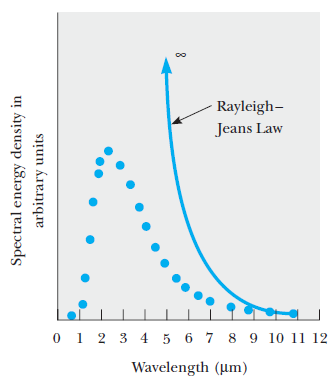
\includegraphics[width = 200pt]{Homework11/fig_3_12.PNG}
    \end{center}
    As is apparent with the graph, these coefficients make complete sense. As you get smaller $\lambda$ your coefficient is going to plummet, as our does for wavelength we divide by 10. When we have a larger $\lambda$ our lines match up, so our coefficient will be close to one, as it is. \faThumbsOUp
\newpage
    
\section*{Problem 3}
    \[\int_{\lambda = 0}^\infty \frac{2\pi hc^2}{\lambda^5 (e^{hc/\lambda k_b T}-1}d\lambda\]
    We can use the substitution:
    \[\frac{hc}{\lambda k_B T} = x \rightarrow \lambda = \frac{hc}{k_B T}\frac{1}{x}\]
    \[d\lambda = -\frac{hc}{k_B T}\frac{1}{x^2}dx\]\\
    
    \[\int_{\lambda = 0}^\infty \frac{2 \pi hc^2}{\Big(\frac{hc}{k_B T}\frac{1}{x}\Big)^5(e^x -1)}\frac{hc}{k_B T}\Big(-\frac{1}{x^2}\Big)dx\]
    \[\lambda = 0 \rightarrow x = \infty; \lambda = \infty \rightarrow x=0\]
    \[\frac{2\pi(K_B T)^T}{h^3 c^2}\int_{x=0}^\infty \frac{x^3}{e^x -1}dx\]

\end{document}
